\documentclass[dvipdfmx,autodetect-engine,titlepage]{jsarticle}
\usepackage[dvipdfm]{graphicx}
\usepackage{ascmac}
\usepackage{fancybox}
\usepackage{listings}
\usepackage{plistings}
\usepackage{itembkbx}
\usepackage{amsmath}
\usepackage{amssymb}
\usepackage{amsfonts}
\usepackage{svg}
\usepackage{url}
\usepackage{graphics}
\usepackage{multirow}
\usepackage{listings,jvlisting}

\textheight=23cm
\renewcommand{\figurename}{図}
\renewcommand{\tablename}{表}
\newenvironment{code}
{\vspace{0.5zw}\VerbatimEnvironment  
\begin{screen} 
\baselineskip=1.0\normalbaselineskip
 \begin{Verbatim}}
{\end{Verbatim}
\baselineskip=\normalbaselineskip
 \end{screen}\vspace{0.5zw}} 

\title{情報理工学部 SNコース 3回\\
リレーショナルデータベースにおけるモデリング\\}
\author{2600200443-6\\Yamashita Kyohei\\山下 恭平}
\date{Jun 19 2022}

\begin{document}

\maketitle

% \section{データベースについて}

% 問題文中で与えられた表は、Exel的に表現おり、元のリレーショナルデータベースとは
% 異なる形をしているので、元の形に一度戻してみると、以下のようになると考えられる。
% \begin{table}[h]
%   \centering
%   \begin{tabular}{cccccrrr}
%   \hline
%   \multicolumn{1}{|c|}{顧客ID}                  & \multicolumn{1}{c|}{顧客名}                   & \multicolumn{1}{c|}{所在地}                  & \multicolumn{1}{c|}{商品ID} & \multicolumn{1}{c|}{商品名}    & \multicolumn{1}{l|}{単価}  & \multicolumn{1}{l|}{個数}  & \multicolumn{1}{l|}{価格合計}                   \\ \hline\hline
%   \multicolumn{1}{|c|}{A001}                  & \multicolumn{1}{c|}{大津電子}                  & \multicolumn{1}{c|}{大津市}                  & \multicolumn{1}{c|}{1010} & \multicolumn{1}{c|}{3mm ネジ} & \multicolumn{1}{r|}{10}  & \multicolumn{1}{r|}{300} & \multicolumn{1}{r|}{3000}                   \\ \hline
%   \multicolumn{1}{|c|}{A001}                  & \multicolumn{1}{c|}{大津電子}                  & \multicolumn{1}{c|}{大津市}                  & \multicolumn{1}{c|}{1011} & \multicolumn{1}{c|}{丸形プラグ}  & \multicolumn{1}{r|}{200} & \multicolumn{1}{r|}{150} & \multicolumn{1}{r|}{30000}                  \\ \hline
%   \multicolumn{1}{|c|}{A002}                  & \multicolumn{1}{c|}{草津精工}                  & \multicolumn{1}{c|}{草津市}                  & \multicolumn{1}{c|}{1010} & \multicolumn{1}{c|}{3mm ネジ} & \multicolumn{1}{r|}{10}  & \multicolumn{1}{r|}{200} & \multicolumn{1}{r|}{2000}                   \\ \hline
%   \multicolumn{1}{|c|}{A002}                  & \multicolumn{1}{c|}{草津精工}                  & \multicolumn{1}{c|}{草津市}                  & \multicolumn{1}{c|}{1011} & \multicolumn{1}{c|}{丸形プラグ}  & \multicolumn{1}{r|}{200} & \multicolumn{1}{r|}{120} & \multicolumn{1}{r|}{24000}                  \\ \hline
%   \multicolumn{1}{|c|}{A002}                  & \multicolumn{1}{c|}{草津精工}                  & \multicolumn{1}{c|}{草津市}                  & \multicolumn{1}{c|}{1045} & \multicolumn{1}{c|}{5m 銅線}  & \multicolumn{1}{r|}{500} & \multicolumn{1}{r|}{50}  & \multicolumn{1}{r|}{25000}                  \\ \hline
%   \multicolumn{1}{l}{}                        & \multicolumn{1}{l}{}                       & \multicolumn{1}{l}{}                      & \multicolumn{1}{l}{}      & \multicolumn{1}{l}{}        & \multicolumn{1}{l}{}     & \multicolumn{1}{l}{}     & \multicolumn{1}{l}{}                        \\
%                                               &                                            & \multicolumn{3}{c}{↓Exelなどによるセル結合}                                                                  & \multicolumn{1}{l}{}     & \multicolumn{1}{l}{}     & \multicolumn{1}{l}{}                        \\
%                                               &                                            &                                           &                           &                             &                          &                          &                                             \\ \hline
%   \multicolumn{1}{|c|}{顧客ID}                  & \multicolumn{1}{c|}{顧客名}                   & \multicolumn{1}{c|}{所在地}                  & \multicolumn{1}{c|}{商品ID} & \multicolumn{1}{c|}{商品名}    & \multicolumn{1}{l|}{単価}  & \multicolumn{1}{l|}{個数}  & \multicolumn{1}{l|}{価格合計}                   \\ \hline\hline
%   \multicolumn{1}{|c|}{\multirow{2}{*}{A001}} & \multicolumn{1}{c|}{\multirow{2}{*}{大津電子}} & \multicolumn{1}{c|}{\multirow{2}{*}{大津市}} & \multicolumn{1}{c|}{1010} & \multicolumn{1}{c|}{3mm ネジ} & \multicolumn{1}{r|}{10}  & \multicolumn{1}{r|}{300} & \multicolumn{1}{r|}{\multirow{2}{*}{33000}} \\ \cline{4-7}
%   \multicolumn{1}{|c|}{}                      & \multicolumn{1}{c|}{}                      & \multicolumn{1}{c|}{}                     & \multicolumn{1}{c|}{1011} & \multicolumn{1}{c|}{丸形プラグ}  & \multicolumn{1}{r|}{200} & \multicolumn{1}{r|}{150} & \multicolumn{1}{r|}{}                       \\ \hline
%   \multicolumn{1}{|c|}{\multirow{3}{*}{A002}} & \multicolumn{1}{c|}{\multirow{3}{*}{草津精工}} & \multicolumn{1}{c|}{\multirow{3}{*}{草津市}} & \multicolumn{1}{c|}{1010} & \multicolumn{1}{c|}{3mm ネジ} & \multicolumn{1}{r|}{10}  & \multicolumn{1}{r|}{200} & \multicolumn{1}{r|}{\multirow{3}{*}{51000}} \\ \cline{4-7}
%   \multicolumn{1}{|c|}{}                      & \multicolumn{1}{c|}{}                      & \multicolumn{1}{c|}{}                     & \multicolumn{1}{c|}{1011} & \multicolumn{1}{c|}{丸形プラグ}  & \multicolumn{1}{r|}{200} & \multicolumn{1}{r|}{120} & \multicolumn{1}{r|}{}                       \\ \cline{4-7}
%   \multicolumn{1}{|c|}{}                      & \multicolumn{1}{c|}{}                      & \multicolumn{1}{c|}{}                     & \multicolumn{1}{c|}{1045} & \multicolumn{1}{c|}{5m 銅線}  & \multicolumn{1}{r|}{500} & \multicolumn{1}{r|}{50}  & \multicolumn{1}{r|}{}                       \\ \hline
%   \end{tabular}
%   \end{table}

% この課題では、セル結合前の表をもとに考えることにする。

\section{どのような関数従属性が存在しているか}

このスキーマには以下の3つの関数従属性が考えられる。

\begin{quote}
  \begin{itemize}
   \item 顧客ID → 顧客名 , 所在地
   \item 商品ID → 商品名 , 単価
   \item 顧客ID , 商品ID → 個数 , 合計価格
  \end{itemize}
 \end{quote}

 一つ目の「顧客ID → 顧客名 , 所在地」を考えた時、「顧客名 → 顧客ID , 所在地」
 も考えられるが、もし同名の顧客が存在した場合に正しく結果を得られることができない。
 また、「顧客名 , 所在地 → 顧客ID」の場合についても、同名かつ所在地が同じだった
 場合にエラーが発生する。\\
 二つ目の「商品ID → 商品名 , 単価」を考える。企業のデータベースであるので
 商品名が一致することはないと考えられる。この時「商品ID → 商品名 → 単価」の
 推移的関数従属があるように見えるが、\\「商品ID \begin{math}\leftrightarrows \end{math} 商品名」
 の関係が存在するので、推移的関数従属はないと考えられる、ここで、商品IDをキー
 とする理由は、商品名が変更になった際のエラーを防ぐためである。\\
 三つ目では、一つ目と同様の理由で、個数と商品価格が一致したときにエラーが発生するので
 ID二つをキーとする。

\section{キーは何か}

第一正規系のとき、それぞれの関数従属性よりキーは(顧客ID,商品ID)の二つである。\\

上の問題で示した、3つそれぞれの関数従属についてテーブルを作成したと考え、Kを
キー属性、FKを外部キーとすると以下の図のようになる。

\begin{figure}[htbp]
  \begin{minipage}{0.33\hsize}
   \begin{center}
    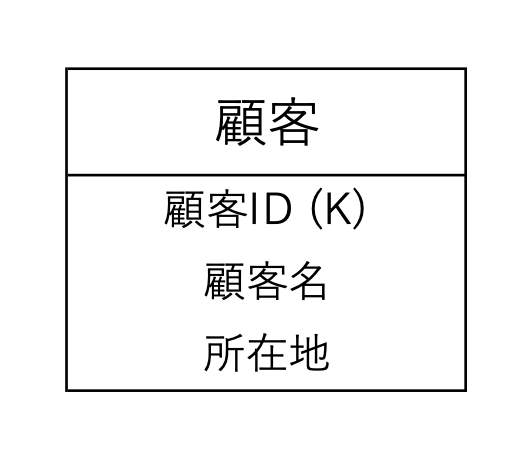
\includegraphics[width=40mm]{pic1.png}
   \end{center}
   \label{fig:one}
  \end{minipage}
  \begin{minipage}{0.33\hsize}
  \begin{center}
   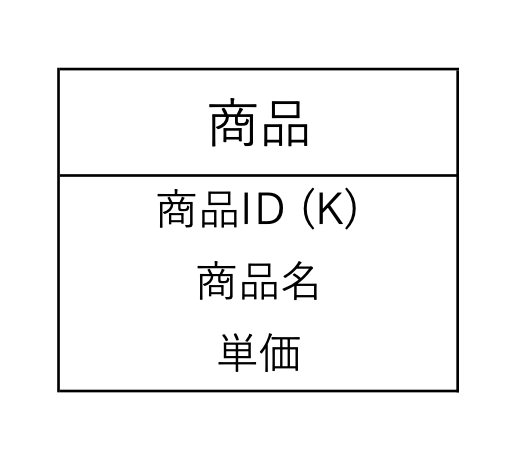
\includegraphics[width=40mm]{pic2.png}
  \end{center}
   \label{fig:two}
  \end{minipage}
  \begin{minipage}{0.33\hsize}
  \begin{center}
   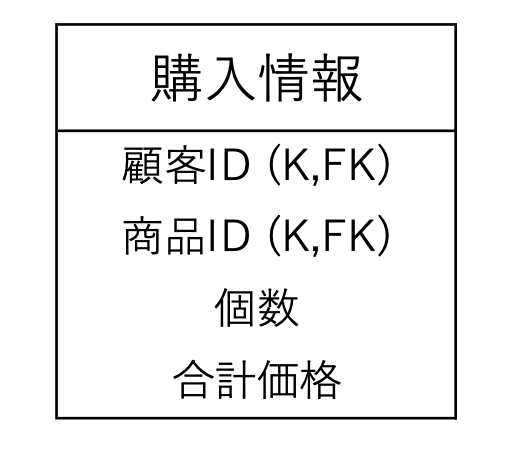
\includegraphics[width=40mm]{pic3.png}
  \end{center}
   \label{fig:three}
  \end{minipage}
 \end{figure}

 \newpage

\section{どの正規化のレベルを満たしているか}

主キーが全てのテーブルで一致しているので、一つにまとめることができる。
このときは、第一正規系となる。関数従属に基づき、テーブルを分解した場合は第三正規系となる。

\begin{table}[h]
  \centering
  \caption{第一正規系}
  \begin{tabular}{|c|c|c|c|c|r|r|r|}
  \hline
  顧客ID & 顧客名  & 所在地 & 商品ID & 商品名    & \multicolumn{1}{l|}{単価} & \multicolumn{1}{l|}{個数} & \multicolumn{1}{l|}{価格合計} \\ \hline\hline
  A001 & 大津電子 & 大津市 & 1010 & 3mm ネジ & 10                      & 300                     & 3000                      \\ \hline
  A001 & 大津電子 & 大津市 & 1011 & 丸形プラグ  & 200                     & 150                     & 30000                     \\ \hline
  A002 & 草津精工 & 草津市 & 1010 & 3mm ネジ & 10                      & 200                     & 2000                      \\ \hline
  A002 & 草津精工 & 草津市 & 1011 & 丸形プラグ  & 200                     & 120                     & 24000                     \\ \hline
  A002 & 草津精工 & 草津市 & 1045 & 5m 銅線  & 500                     & 50                      & 25000                     \\ \hline
  \end{tabular}
  \end{table}

\begin{table}[h]
  \centering
  \caption{第三正規系}
  \begin{tabular}{llllllll|l|l|l|l|}
  \cline{1-3} \cline{5-7} \cline{9-12}
  \multicolumn{1}{|l|}{顧客ID} & \multicolumn{1}{l|}{顧客名}  & \multicolumn{1}{l|}{所在地} & \multicolumn{1}{l|}{} & \multicolumn{1}{l|}{商品ID} & \multicolumn{1}{l|}{商品名}    & \multicolumn{1}{l|}{単価}  &  & 顧客ID & 商品ID & 個数  & 価格合計  \\ \cline{1-3} \cline{5-7} \cline{9-12} 
  \multicolumn{1}{|l|}{A001} & \multicolumn{1}{l|}{大津電子} & \multicolumn{1}{l|}{大津市} & \multicolumn{1}{l|}{} & \multicolumn{1}{l|}{1010} & \multicolumn{1}{l|}{3mm ネジ} & \multicolumn{1}{l|}{10}  &  & A001 & 1010 & 300 & 3000  \\ \cline{1-3} \cline{5-7} \cline{9-12} 
  \multicolumn{1}{|l|}{A002} & \multicolumn{1}{l|}{草津精工} & \multicolumn{1}{l|}{草津市} & \multicolumn{1}{l|}{} & \multicolumn{1}{l|}{1011} & \multicolumn{1}{l|}{丸形プラグ}  & \multicolumn{1}{l|}{200} &  & A001 & 1011 & 150 & 30000 \\ \cline{1-3} \cline{5-7} \cline{9-12} 
                             &                           &                          & \multicolumn{1}{l|}{} & \multicolumn{1}{l|}{1045} & \multicolumn{1}{l|}{5m 銅線}  & \multicolumn{1}{l|}{500} &  & A002 & 1010 & 200 & 2000  \\ \cline{5-7} \cline{9-12} 
                             &                           &                          &                       &                           &                             &                          &  & A002 & 1011 & 120 & 24000 \\ \cline{9-12} 
                             &                           &                          &                       &                           &                             &                          &  & A002 & 1045 & 50  & 25000 \\ \cline{9-12} 
  \end{tabular}
  \end{table}

\section{BCNFになるように分解せよ}

第三正規系の形の時、「商品ID \begin{math}\leftrightarrows \end{math} 商品名」が存在しており、
非キー属性から、主キー属性への関数従属が存在したので、これを無くせばボイスコッド正規系
となる。以下は、ボイスコッド正規系で分解したものである。ここで、(主)は主キーを、(外)は
外部キーを表す。

\begin{table}[h]
  \centering
  \begin{tabular}{cllccclll}
  \cline{1-3} \cline{5-8}
  \multicolumn{1}{|c|}{顧客ID(主)}   & \multicolumn{1}{c|}{顧客名}  & \multicolumn{1}{c|}{所在地} & \multicolumn{1}{c|}{} & \multicolumn{1}{c|}{顧客ID(主,外)} & \multicolumn{1}{c|}{商品ID(主,外)} & \multicolumn{1}{c|}{個数}  & \multicolumn{1}{c|}{価格合計}  &                      \\ \cline{1-3} \cline{5-8}
  \multicolumn{1}{|c|}{A001}      & \multicolumn{1}{l|}{大津電子} & \multicolumn{1}{l|}{大津市} & \multicolumn{1}{l|}{} & \multicolumn{1}{c|}{A001}      & \multicolumn{1}{c|}{1010}      & \multicolumn{1}{r|}{300} & \multicolumn{1}{r|}{3000}  & \multicolumn{1}{c}{} \\ \cline{1-3} \cline{5-8}
  \multicolumn{1}{|c|}{A002}      & \multicolumn{1}{l|}{草津精工} & \multicolumn{1}{l|}{草津市} & \multicolumn{1}{l|}{} & \multicolumn{1}{c|}{A001}      & \multicolumn{1}{c|}{1011}      & \multicolumn{1}{r|}{150} & \multicolumn{1}{r|}{30000} & \multicolumn{1}{c}{} \\ \cline{1-3} \cline{5-8}
  \multicolumn{1}{l}{}            &                           &                          & \multicolumn{1}{l|}{} & \multicolumn{1}{c|}{A002}      & \multicolumn{1}{c|}{1010}      & \multicolumn{1}{r|}{200} & \multicolumn{1}{r|}{2000}  & \multicolumn{1}{c}{} \\ \cline{5-8}
  \multicolumn{1}{l}{}            &                           &                          & \multicolumn{1}{l|}{} & \multicolumn{1}{c|}{A002}      & \multicolumn{1}{c|}{1011}      & \multicolumn{1}{r|}{120} & \multicolumn{1}{r|}{24000} & \multicolumn{1}{c}{} \\ \cline{5-8}
                                  & \multicolumn{1}{c}{}      &                          & \multicolumn{1}{c|}{} & \multicolumn{1}{c|}{A002}      & \multicolumn{1}{c|}{1045}      & \multicolumn{1}{r|}{50}  & \multicolumn{1}{r|}{25000} & \multicolumn{1}{c}{} \\ \cline{5-8}
                                  & \multicolumn{1}{r}{}      &                          &                       &                                & \multicolumn{1}{l}{}           &                          &                            &                      \\ \cline{1-2} \cline{5-6}
  \multicolumn{1}{|c|}{商品ID(主,外)} & \multicolumn{1}{c|}{単価}   & \multicolumn{1}{c}{}     & \multicolumn{1}{c|}{} & \multicolumn{1}{c|}{商品ID(主)}   & \multicolumn{1}{c|}{商品名(主)}    &                          &                            &                      \\ \cline{1-2} \cline{5-6}
  \multicolumn{1}{|c|}{1010}      & \multicolumn{1}{r|}{10}   & \multicolumn{1}{r}{}     & \multicolumn{1}{c|}{} & \multicolumn{1}{c|}{1010}      & \multicolumn{1}{c|}{3mm ネジ}    &                          &                            &                      \\ \cline{1-2} \cline{5-6}
  \multicolumn{1}{|c|}{1011}      & \multicolumn{1}{r|}{200}  & \multicolumn{1}{r}{}     & \multicolumn{1}{c|}{} & \multicolumn{1}{c|}{1011}      & \multicolumn{1}{c|}{丸形プラグ}     &                          &                            &                      \\ \cline{1-2} \cline{5-6}
  \multicolumn{1}{|c|}{1045}      & \multicolumn{1}{r|}{500}  & \multicolumn{1}{r}{}     & \multicolumn{1}{c|}{} & \multicolumn{1}{c|}{1045}      & \multicolumn{1}{c|}{5m 銅線}     &                          &                            &                      \\ \cline{1-2} \cline{5-6}
  \end{tabular}
  \end{table}

\section{BCNFに分解したあとに構築する索引の検討}

商品単価で検索範囲を絞りたいので、(商品ID、単価)を持つテーブルに対して、
属性「単価」へB+木構造を持つ索引を付与することで、指定された範囲の単価を持つ、
商品IDを通常より早く探索することができる。

\section{「価格合計」の冗長性と、それに伴い発生する不整合についての検討}

ここでの価格合計は、あらかじめ価格合計を計算しておき、データベースに格納した
ものと考えられ、「単価 \begin{math}\times\end{math}個数」で求めれるので、
冗長性を保つといえる。しかし、何らかの原因で単価の値が更新されたとき、格納
されている値と、計算で得られる値が一致せず、不整合が発生すると考えられる。

\end{document}